\documentclass{standalone}
\usepackage{tikz}
\usetikzlibrary{fit,chains,arrows,positioning,calc}
\renewcommand{\familydefault}{\sfdefault}

\begin{document}
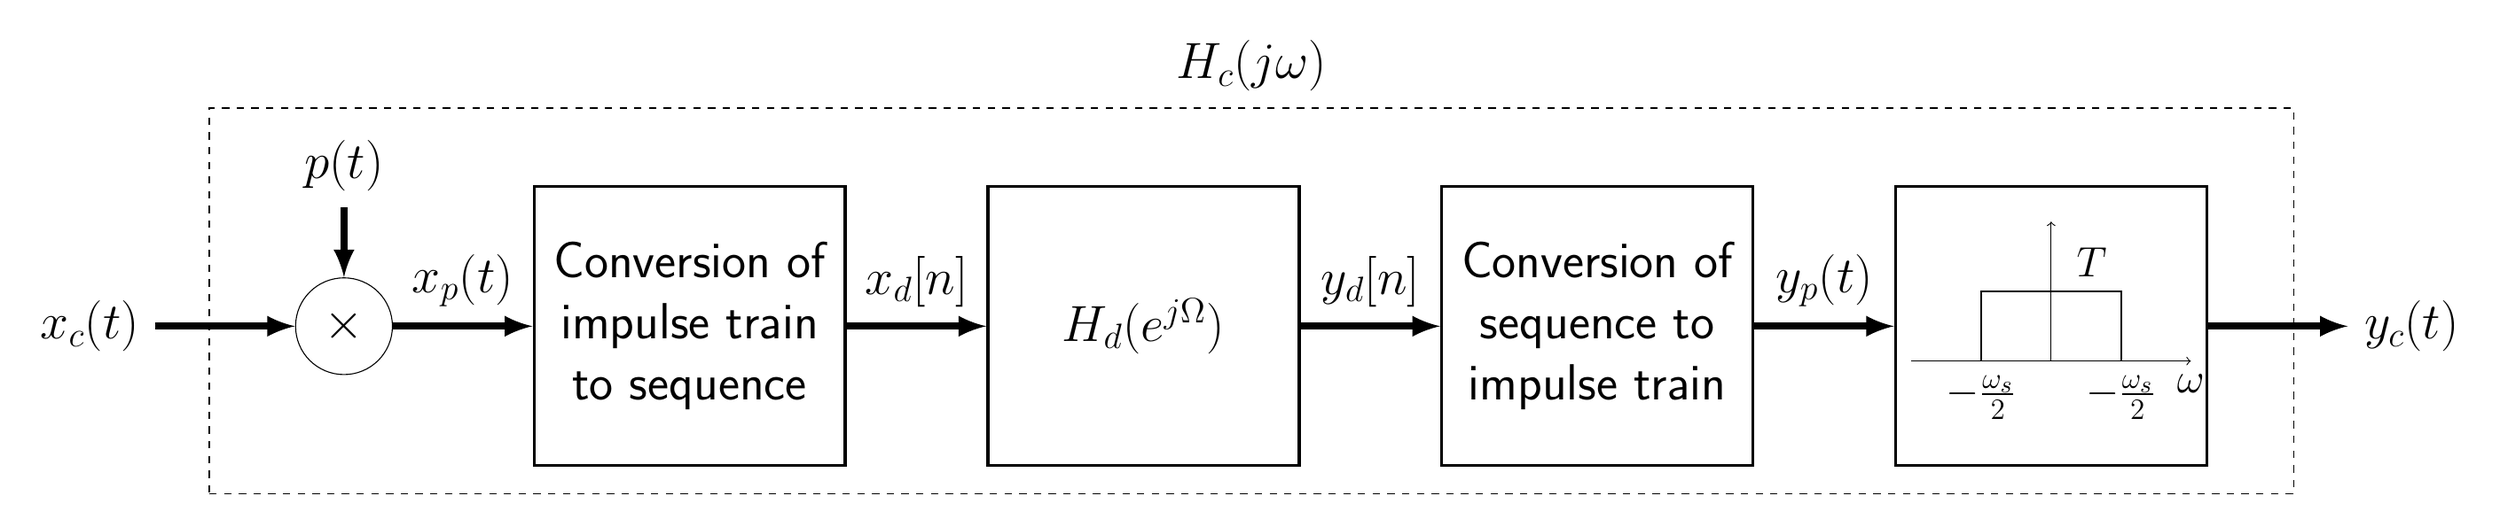
\begin{tikzpicture}[auto]
    \tikzset{mysymbol/.pic={
    \LARGE
    \draw[->] (-2, 0) -- (2, 0) node[below] {$\omega$} ;
    \draw[->] (0, 0) -- (0, 2);
    \draw[thick] (-1, 0) node[below] {$-\frac{\omega_s}{2}$} -- (-1, 1)  -- (1, 1) node[above left] {$T$} -- (1, 0) node[below] {$-\frac{\omega_s}{2}$} ;
}}
    \huge

    \node (box1) {$x_c(t)$};
    \node[draw, circle, right=2cm of box1] (box2) {$\times$};
    \begin{scope}[start chain=going right, node distance=2cm, every node/.style={draw, on chain, minimum size=4cm, text width=4cm, text centered, very thick}]
    \node[right=of box2] (box3) {Conversion of impulse train to sequence};
    \node (box4) {$H_d(e^{j\Omega})$};
    \node (box5) {Conversion of sequence to impulse train};
    % \node (boxplot){\usebox{\boxplot}};
    \node[draw] (boxplot){};
    \end{scope}
    \pic at ([yshift=-0.5cm]boxplot) {mysymbol};
    \node[right=2cm of boxplot] (box7) {$y_c(t)$};
    \node[above=of box2] (up) {$p(t)$};
    \node[below=of box2] (down) {};
    \draw[-latex, line width=1mm]
        (box1) edge node[above right] (e1) {} (box2)
        (box2) edge node[above] (e2) {$x_p(t)$} (box3)
        (box3) edge node[above] (e3) {$x_d[n]$} (box4)
        (box4) edge node[above] (e4) {$y_d[n]$} (box5)
        (box5) edge node[above] (e5) {$y_p(t)$} (boxplot)
        (boxplot) edge node[above left] (e6) {} (box7)
        (up) edge (box2)
        ;
    \node[fit=(e1) (box2) (box3) (up) (down) (e6), draw, dashed, label=$H_c(j\omega)$] {};
\end{tikzpicture}

\end{document}

